\section{Results}
\label{exp}
We first evaluate our approach, which we denote as \textbf{Sample View Clean (SVC)}, on a synthetic benchmark dataset where we can control the data distribution and the update rate.
Next, we evaluate overheads and tradeoffs to using our approach.
Then, we evaluate the benefits and tradeoffs of outlier indexing.
After evaluation on the benchmark, we present an end-to-end application of log analysis with a dataset from a video streaming company.

\begin{figure*}[ht!]
\hspace{-5.5em}
 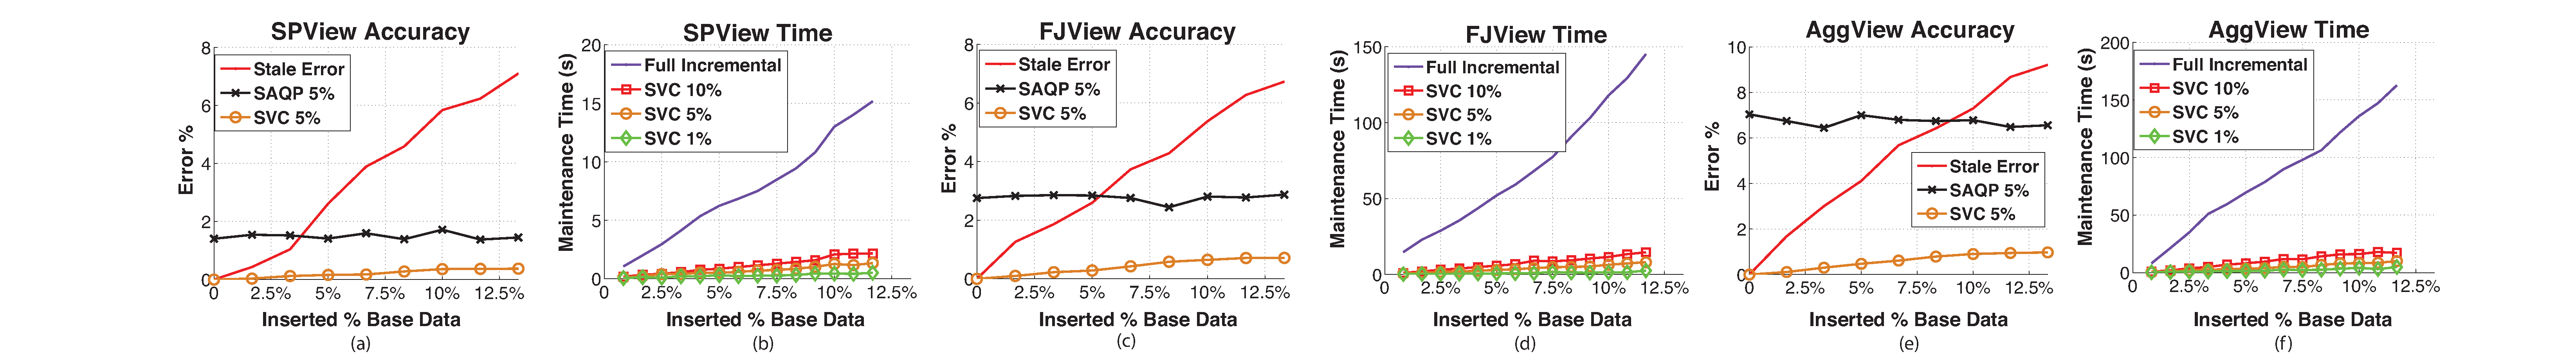
\includegraphics[scale=0.19]{exp/exp2-full.eps}
 \caption{For each of the three views listed above, we plot the accuracy for 5\% samples compared to SAQP and a stale baseline. We also plot the maintenance time for each of the views in comparison to full incremental maintenance for a 1\%, 5\% and 10\% sample. \label{exp2update} }
\end{figure*}

\subsection{Experimental Setting}
\subsubsection{TPCD-Skew}
{\noindent \bf Dataset Description and Views :}
TPCD-Skew dataset \cite{tpcdskew} is based on the Transaction Processing Council's benchmark
schema but is modified so that it generates a dataset with values drawn from a Zipfian distribution instead of uniformly.
The Zipfian distribution \cite{mitzenmacher2004brief} is a long-tailed distribution with a single parameter $z=\{0,1,2,3,4\}$ which a larger
value means a more extreme tail.
This dataset has been applied to benchmark other sampling based approaches, approximate queries, and outlier performance \cite{chaudhuri2001overcoming, agrawal2005database}.
The base dataset is 10GB corresponding to 60M records.
Unless otherwise noted, we experiment with $z=2$.
The dataset is provided in the form of a generation program which can generate both the base tables and a set of updates.

For this dataset, we applied our approach to three materialized views, each of a different type:

{\noindent \bf \spview :}
\begin{lstlisting}
SELECT *, 
       IF(Lcase(l_shipinstruct) LIKE '%deliver%' 
          AND Lcase(l_shipmode) LIKE '%air%', 'priority', 'slow') 
FROM   lineitem_s 
\end{lstlisting}

\vspace{0.5em}

{\noindent \bf \aggview :}
\begin{lstlisting}
SELECT l_orderkey, l_shipdate, 
       Sum(l_quantity)      AS quantity_sum, 
       Sum(l_extendedprice) AS extendedprice_sum, 
       Max(l_receiptdate)   AS receiptdate_max, 
       Count(*)             AS group_count 
FROM   lineitem 
GROUP  BY l_orderkey, 
          l_shipdate 
\end{lstlisting}

\vspace{0.5em}

{\noindent \bf \fjview :}
\begin{lstlisting}
SELECT supplier.*, customer.* 
FROM   customer, orders, lineitem, supplier, partsupp 
WHERE  c_custkey = o_custkey 
       AND o_orderkey = l_orderkey 
       AND l_suppkey = ps_suppkey 
       AND l_partkey = ps_partkey 
       AND ps_suppkey = s_suppkey 
       AND s_nationkey <> c_nationkey 
\end{lstlisting}

\vspace{0.5em}

{\noindent \bf Queries on the views :}
Along with the TPCD specification are templates to generate a query workload to benchmark database systems.
We used these templates to generate queries and filtered the query workload to the aggregation queries and the ones whose predicates could be applied on our views.
In all, for each view, we had 10,000 aggregate queries with different randomly generated predicates from the template.

\vspace{0.5em}

{\noindent \bf Experimental Platform :}
All of our experiments for the TPCD-Skew dataset are run on a single r3.large Amazon EC2 node with a MySQL database.
With MySQL, we create these views as tables.
We construct a seperate in-memory temporary table of updates, and then measure the time needed to propagate the neccessary updates (forming the delta table and writing the updates) to the views.
In evaluating \fjview, we only insert records into the lineitem table and create an index on all of the dimension tables.
For \aggview, we have an index on the group by key of sampled materialized view.
Note, that we do not assume there are any indices on the newly inserted records.
We use the MySQL query profiling feature to isolate the cost of view maintenance in both the delta view phase and the refresh phase.

\subsubsection{Conviva}
{\noindent \bf Dataset Description :}
Conviva is a video streaming company and we evaluated our approach on user activity logs \cite{conviva}.
We experimented with a 1TB dataset of these logs which formed a single base table.
With this dataset, there was a corresponding dataset of analyst SQL queries on the log table.
Using the query dataset, we constructed 67 aggregation views and queries to run on the views.
We constructed the queries in a similar way to the TPCD-Skew queries, where we found all of the aggregate queries and filtered down
to those that could run on the views.
We used this dataset to evaluate the end-to-end accuracy and performance of the system on a real dataset and query workload.

\vspace{0.5em}

{\noindent \bf Experimental Platform :}
We evaluated performance on Apache Spark with a 20 node r3.large Amazon EC2 cluster. 
Spark supports materialized views through a distributed data structure called an RDD.
There is a SQL interface which transforms the RDD's using Map-Reduce chains.
The RDD's are immutable, thus requiring significant overhead to maintain.
As Spark does not have support for indices, we rely on partitioned joins for incremental maintenance of the aggregation views.
We partitioned the aggregation views by group-by key, and joined the delta table with the aggregation view.

\subsection{Accuracy}

\subsubsection{Update Rate and Accuracy}
For each of the three views listed above, we evaluate the accuracy of our approach.
We set the sample size to $5\%$ and then vary the number of inserted records by increments of 500K (0.8\% base data) records to a final count of 8M records (13.3\% base data).
For the 10,000 generated queries on the view, we calculate the mean error as a relative percentage of the true value.
As a baseline, we compare against SAQP and no maintenance (ie. the stale error).
In Figure \ref{exp2update}, we show the results of the experiment. 

For all three views a 5\% sample sufficed to acheive a mean relative error of less than 1\%, even though when 8M records were inserted the staleness was 7\%.
Furthermore, in comparision to SAQP, the accuracy our approach is proportional to the amount of correction needed, while SAQP keeps a roughly constant accuracy.
As more records are inserted the approximation error in our approach increases.
However, we find that even for very large amounts of inserted records (>10\% of dataset size), our approach gives significantly more accurate results
than SAQP.
The gain is most pronounced in aggregation views where there are a mixture of updated and inserted rows into the view.
Correcting an update to an existing row is often much smaller than doing so for a new inserted record.

\subsubsection{Sample Size and Accuracy} Next, we explore how sample size affects query results.
We inserted 5M (8\% base data) records, and then vary the sampling ratio for the three types of views and show how much sampling is needed to achieve a given query accuracy.
In Figure \ref{exp1sample}, we show the accuracy as a function of sampling ratio for each of the views.
In our experiment, we found that a 0.1\% sample was sufficient to ensure the approximation error due to sampling was less than the baseline staleness.
SAQP also has this break even point, but we found for this number of inserted records the point SAQP required a much larger sample size.

\begin{figure}[ht!]
\hspace{-4em}
 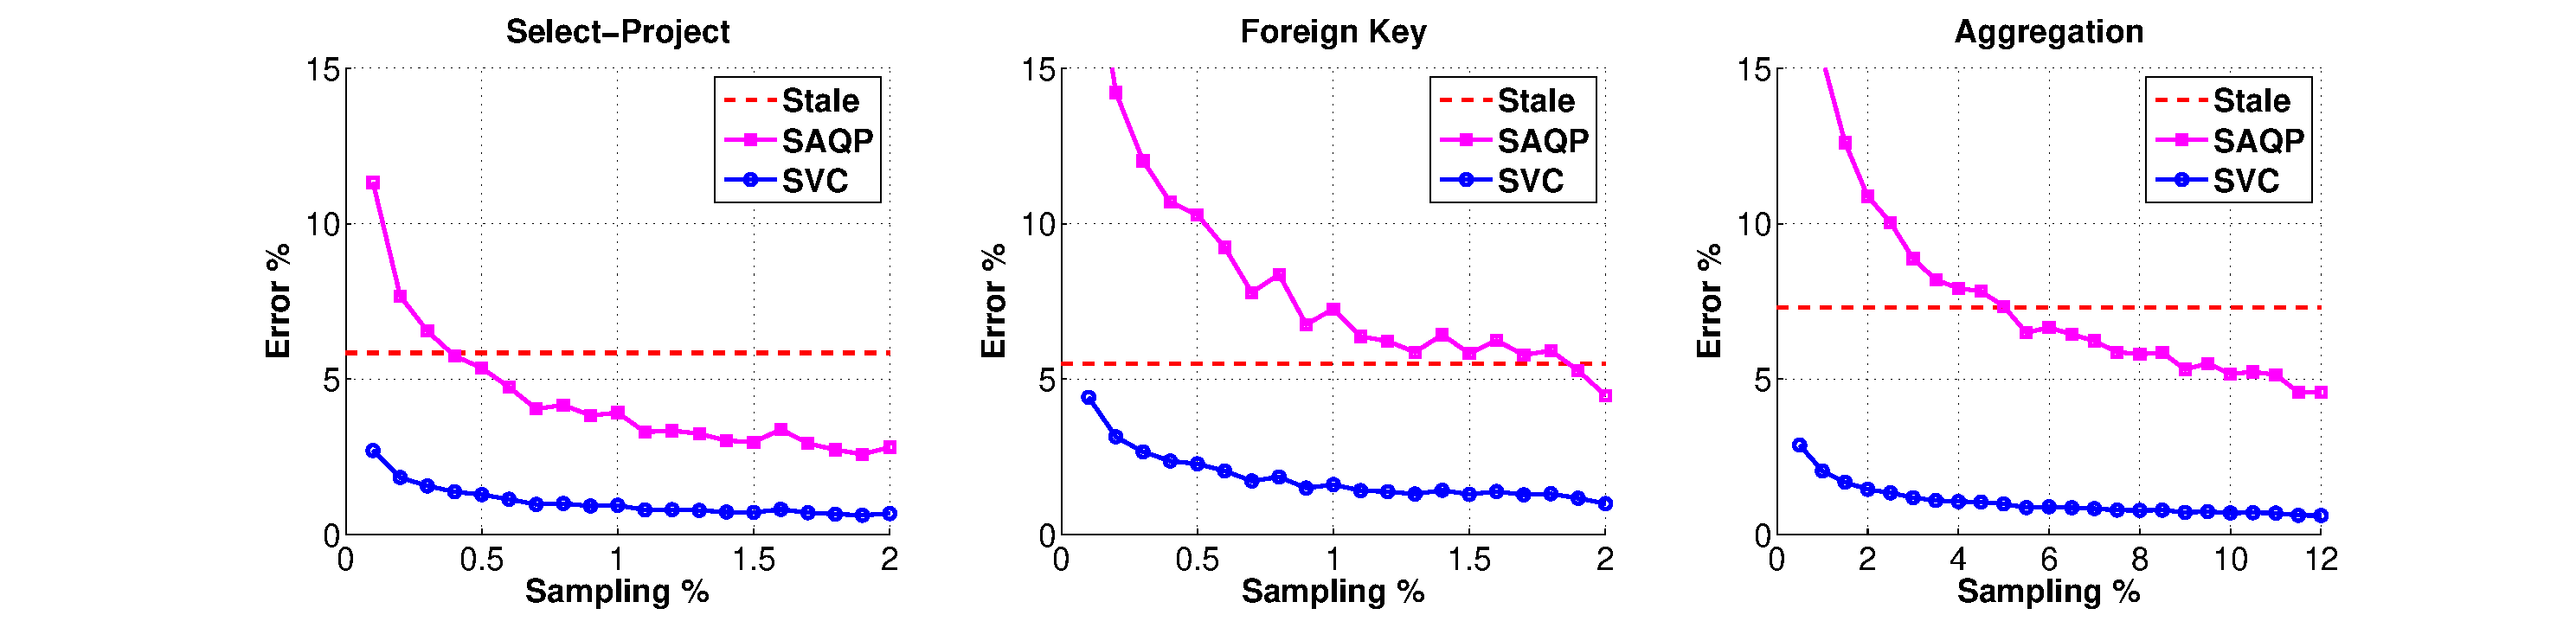
\includegraphics[scale=0.22]{exp/exp1-samplesize-accuracy.eps}
 \caption{As we increase the sample size, the relative error goes down following a $\frac{1}{\sqrt{samplesize}}$ rate. SAQP also follows the same rate so the lines will never cross by only changing the sample size. \label{exp1sample} }
\end{figure}

\subsubsection{Distribution of Query Error} In our earlier experiments, we presented the average error for the queries on the views.
We found that for inserted 5M records (8\% base data) on average querys on the views were 7-9\% stale. 
However, that some queries were much more stale than others.
In this experiment, we looked at the distribution of staleness for the aggregation view.
We used a sampling ratio of 5\% and evaluate the accuracy of our approach. 
In Figure \ref{exp3dist}, we show a CDF of the staleness and a scatter plot comparing the staleness of the query to the accuracy using our correction method.
In the right figure, each green point corresponds to a query with the y-axis as SVC estimation error and the x-axis as staleness. 
Even though some queries are more than 60\% stale, our corrections reduce the relative error to less than 20\%.

\begin{figure}[ht!]
\centering
 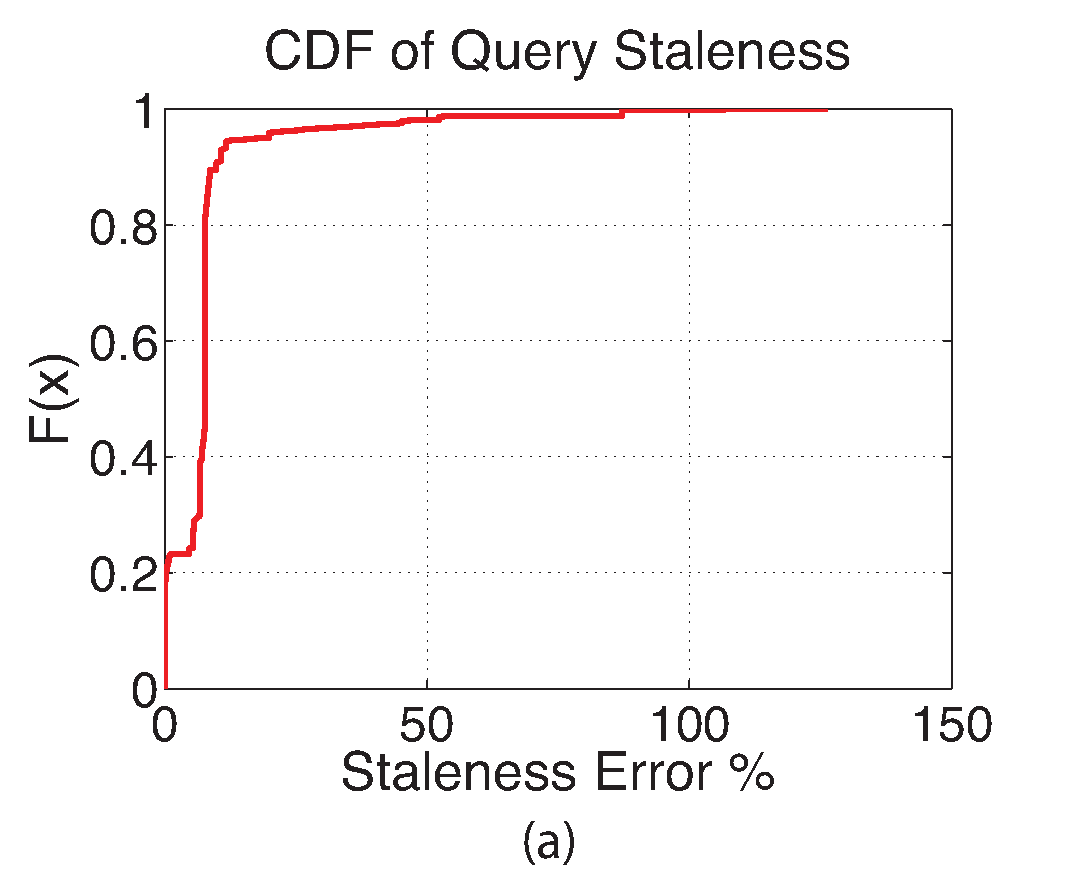
\includegraphics[scale=0.22]{exp/query_error_dist.eps}
 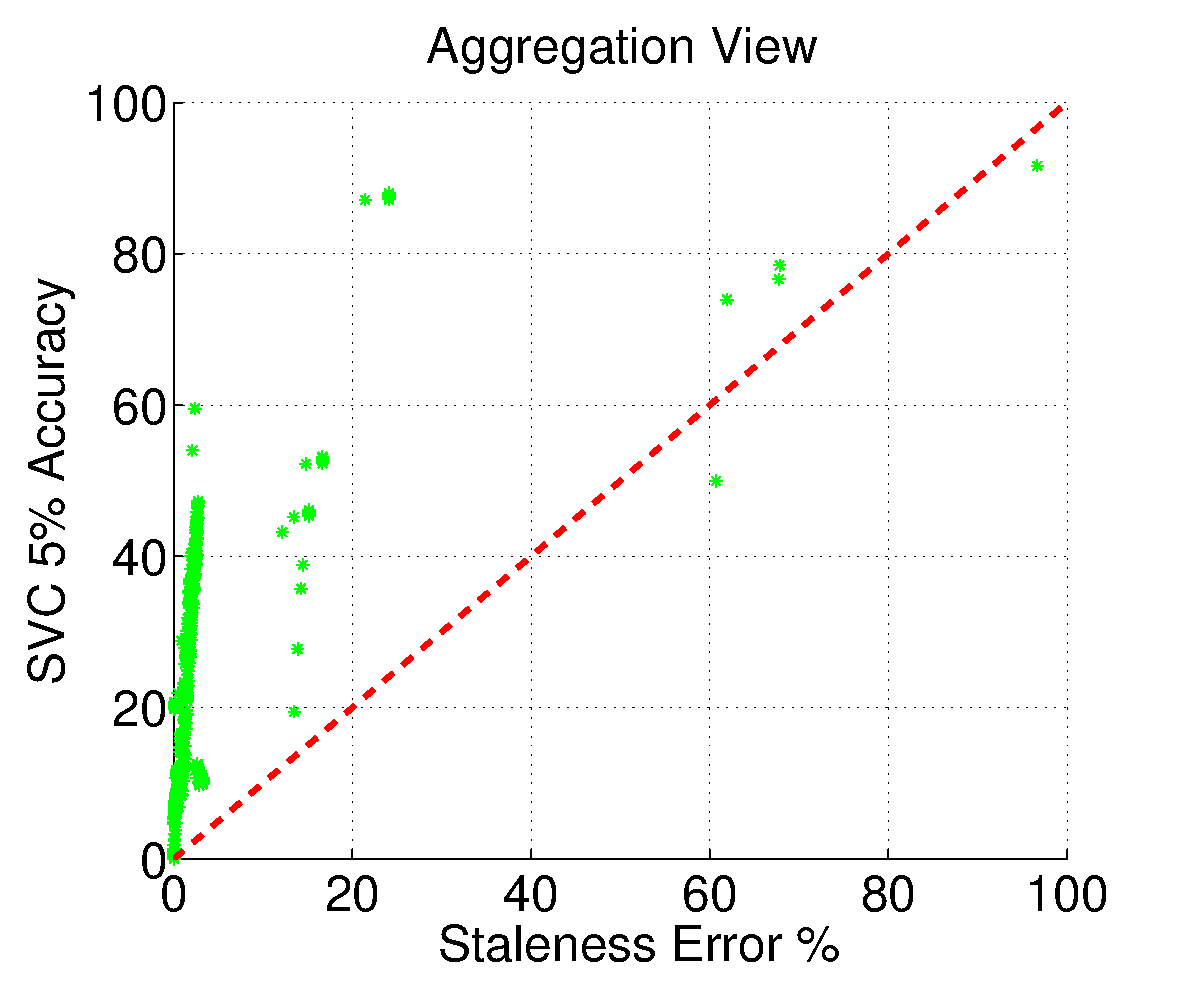
\includegraphics[scale=0.18]{exp/query_error_dist2.eps}
 \caption{While the mean error is 9\%, 5\% of queries have more than 20\% relative error. However, in the second plot, we show a scatter plot of staleness (x-axis) and a query correction accuracy (y-axis). Each green point corresponds to a single query. Points above the dotted line show that we improved query accuracy.\label{exp3dist}}
\end{figure}

The long tail of query errors can occur for a variety of reasons.
First, some of the generated queries are highly selective and a uniform sampling approach may not sample enough records to answer it accurately.
Next, outliers can be caused by large updates to the data that are missed by our sampling, which we will address in subsequent experiments.

\subsection{Efficiency}

\subsubsection{Sampling Efficiency}
In Figure \ref{exp2update}, we evaluate how sampling can reduce maintenance time.
For a batch of updates, we evaluate how long it takes to sample the update patterns as opposed to maintaining the view.
As a baseline, we compare to full incremental maintenance.
We find that for the \aggview and \fjview, which are more expensive to maintain, sampling leads to more pronounced savings. 
For 10\% of data inserted and a 10\% sampling ratio, the maintenance time for \fjview  is 9.35x faster and for \aggview it is 8.4x faster.
However, for the \spview the gains are smaller with a 6.2x speedup.
There are diminishing returns with smaller sample sizes as overheads start becoming significant. 

\subsubsection{Overhead of Query Correction}
In Section \ref{sampling}, we ran cost analyses to argue that sampling can greatly reduce delta view and refresh costs.
In practice, these gains will only be meaningful if the overheads for the query correction are small.
Since, we are correcting a stale query rather than the materialized view, we are shifting some of the computational cost from maintenance time to query execution time.
If our updates only contain insertions, then for \spview and \fjview, since we derive a correction from a sample of the updates, we are guaranteed to have a reduced query time.
However, for aggregation views, query correction requires a scan of the old view and a sample of the maintained view; potentially increasing the time to 
answer the query. 
In our first experiment, we set the sample size to 5\% and evaluate the aggregation view listed earlier for 5M inserted records. 
In Figure \ref{exp10overheads}, we show that average query time is small compared to maintenance time, and furthermore, 
the time to calculate a correction is a just fraction of the query time.
\begin{figure}[h]
\centering
 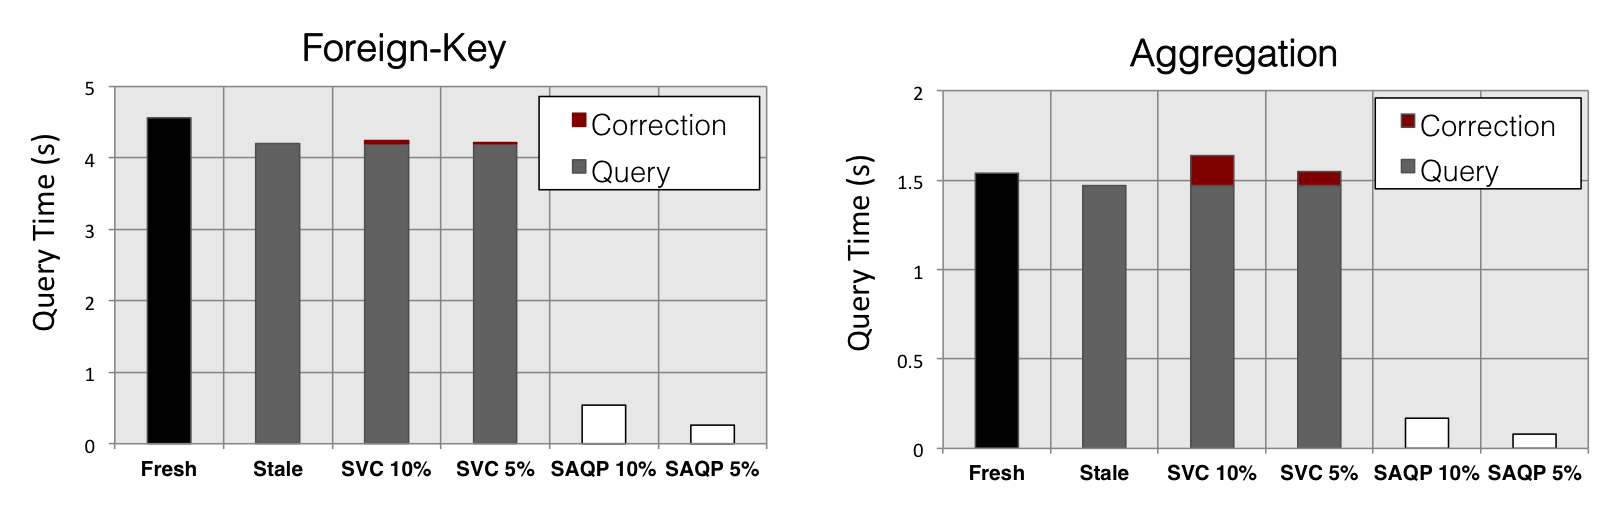
\includegraphics[width=\columnwidth]{exp/total_time_agg_view.png}
 \caption{While, there is an additional overhead to correcting a query, this is small compared to the overall maintenance time. \label{exp10overheads}}
\end{figure}

\subsubsection{View Complexity}
In our maintenance time experiments, we showed that more expensive views tended to benefit from our approach.
We evaluated this tradeoff by taking the simplest possible view, a SELECT of the base table, and then progressively adding clauses to the predicate.
For example:
\begin{lstlisting}
WHERE (condition1)
WHERE (condition1 || condition2)
WHERE (condition1 || condition2 || condition 3)
\end{lstlisting}
We set the sample size to 5\%, insert 5M records (8\% of Base Data), and measure the maintenance time.
For the selection view the only cost for maintenance is a scan of the data and evaluating the predicate. 
Sampling saves on predicate evaluation but introduces the overhead of random number generation (see Section \ref{subsec:pattern}). 
Figure \ref{exp11overheads} illustrates how as the view becomes more complex, the performance improvement given
by our approach increases.
Initially, there is about 5\% overhead, but as the cost of evaluating the benefits increase to a 7.9x speedup over incremental maintenance.
We repeated the same experiment for the aggregation view, but instead we added terms to the group by clause to increase the
cardinality of the view.
We found that for a highly selective group by clause (thus a large view) the savings were 16.9x.
However, when the view was small with the l\_shipdate key, the cost savings were smaller 5.5x.
\begin{figure}[h]
\hspace{-3.5em}
 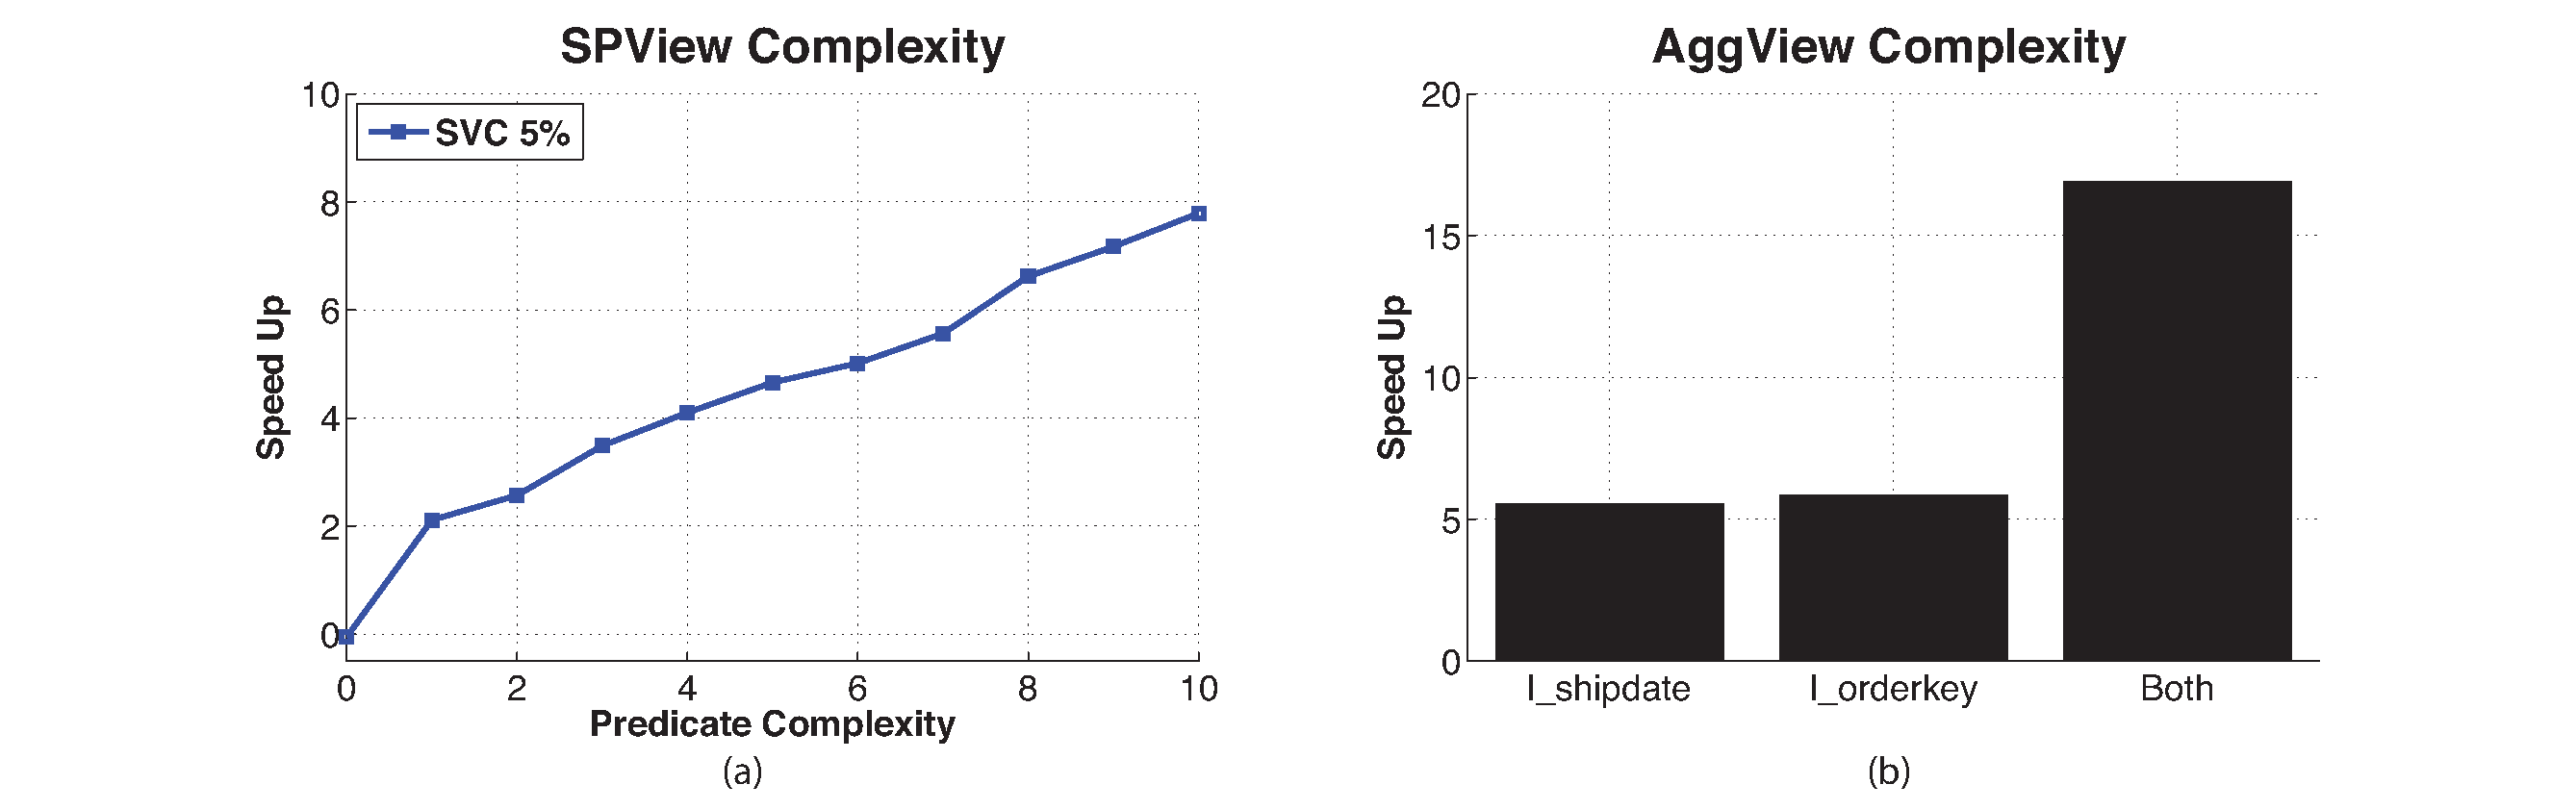
\includegraphics[scale=0.21]{exp/complexity_efficiency_tradeoff.eps}
 \caption{As the views definitions become more complex our approach gives increasing gains. For simplest view (selection no predicate), the overhead is small (5\%).\label{exp11overheads}}
\end{figure}
%This experiment emphasizes that our approach rarely makes performance worse and at worst the improvements are not linear with the sampling ratio.
These experiments emphasize that when views are large and complex, we can have significant improvements.

\subsection{Outlier Indexing}
We use a 5\% sample size and 5M records (8\% of Base Data) inserted, and we evaluate the accuracy of our approach with and without outlier indexing.
We apply the index to the Select-Project view, where we index the attributes l\_extendedprice and l\_quantity.
The results for the other two views were similar, and in this paper, we only present results for the Select-Project views.
We set the outlier index size to the top 500 records in the base table, and looked at the change in accuracy of the top 10 most in accurate query corrections with SVC 5\%.
We find that for these queries, we can improve the accuracy by a factor of 8.2.
We further evaluated the overhead of the approach compared to the base SVC time of 1.44s and found that the overhead was only 1\% for an outlier index of size 1000.
We varied the Zipfian parameter from (0,1,2,3,4), which makes the distribution more skewed, and measured the average improvement in accuracy over all queries.
We found that as the dataset become more skewed, outlier indexing is increasingly important leading to almost a 6x more accurate estimate for $z=4$.

\begin{figure}[ht!]
\hspace{-4em}
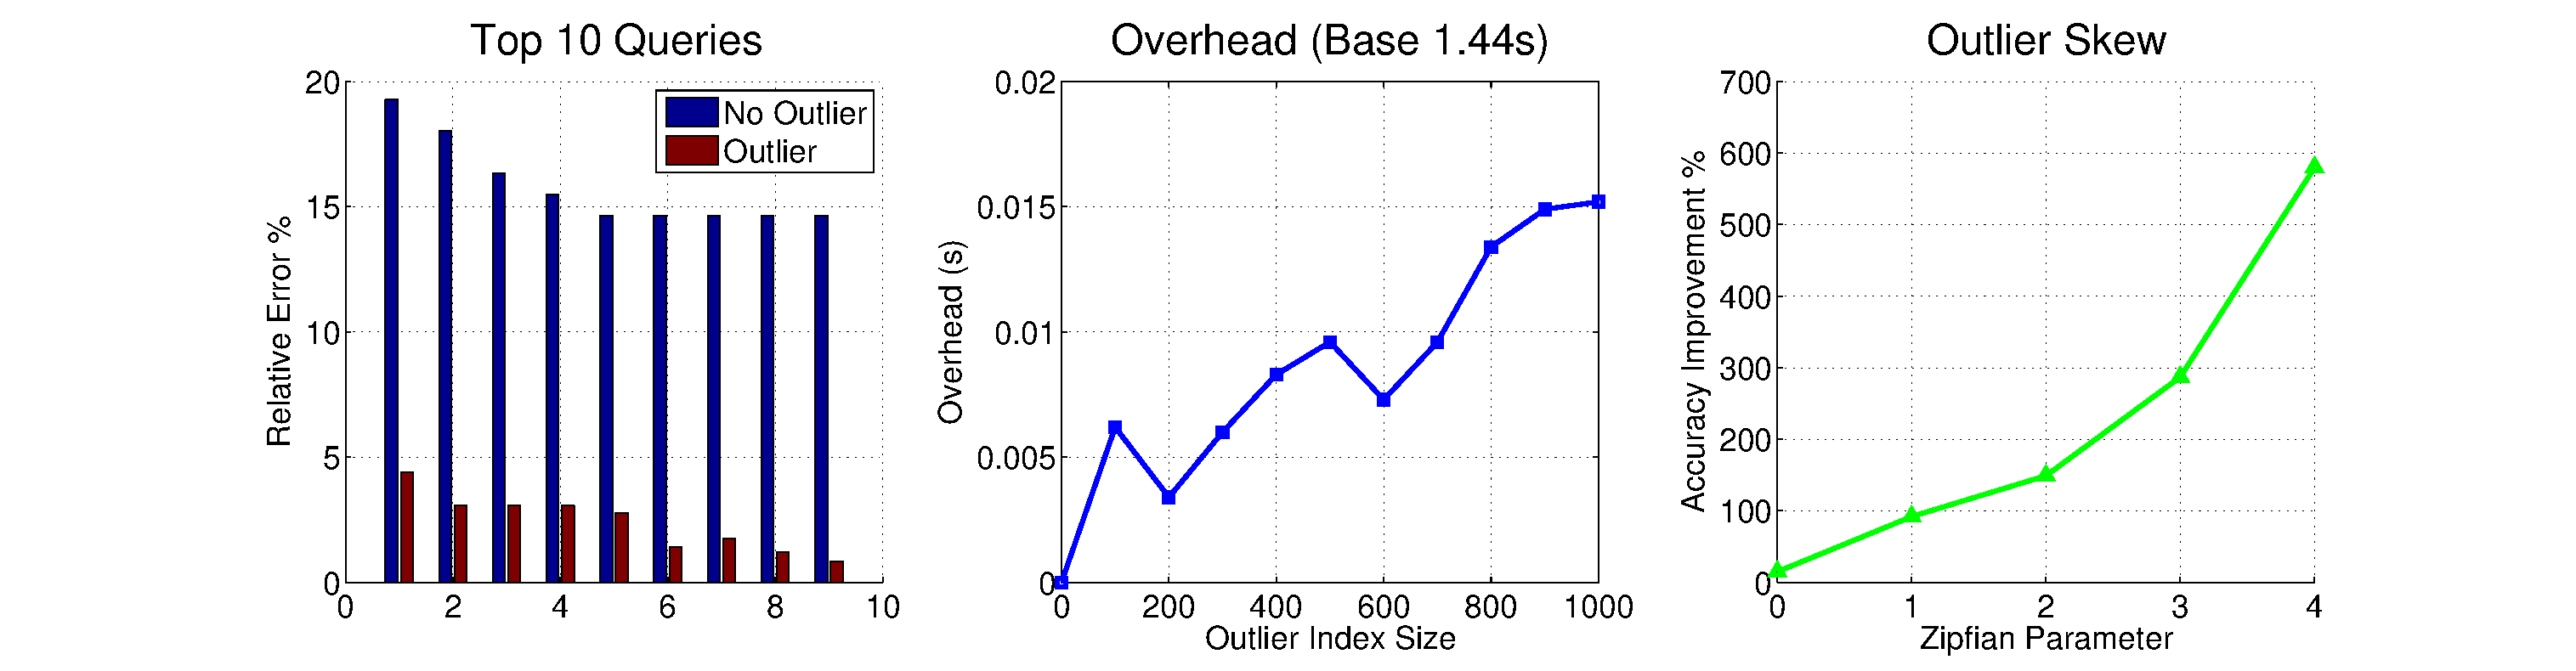
\includegraphics[scale=0.22]{exp/exp6-outlier-full.eps}
 \caption{Outlier indexing greatly improves accuracy of our approach especially in skewed datasets for a small overhead of building the index and ensuring those rows are in the view.\label{exp7outlier}}
\end{figure}

\subsection{Application: Log Analysis For Conviva}
We used a dataset of queries given by Conviva to generate three materialized views.
All three of these views are aggregation views, and for confidentiality, we exclude the actual definitions of the views.
LargeView has the most selective group by clause and was chosen to a be a large view where most of the maintenance is in the form of new rows to insert.
LargeView aggregates session times for each visitor and video pair.
MediumView is a medium size view where maintenance is a mix of both updates and insertions.
MediumView computes buffering time statistics for each visitor over all videos they watched.
SmallView is a small view where most of the maintenance is updates to existing rows.
SmallView computes statistics for log events that triggered error states.

\subsubsection{Representativeness of the Views}
We selected these views to be representative of the dataset and query workload. 
We first present an experiment illustrating where these materialized views lie in the space of all the generated views from the conviva query log.
We derived each view from a 7GB base table and inserted 1.1GB (15\%) of records to the table. 
In Figure \ref{exp12conviva}, we plot the average staleness of each of the views and mark the three views.
While queries on LargeView and MediumView are 21\% and 16\% stale respectively, queries on SmallView are 0.5\%.
\begin{figure}[ht!]
\centering
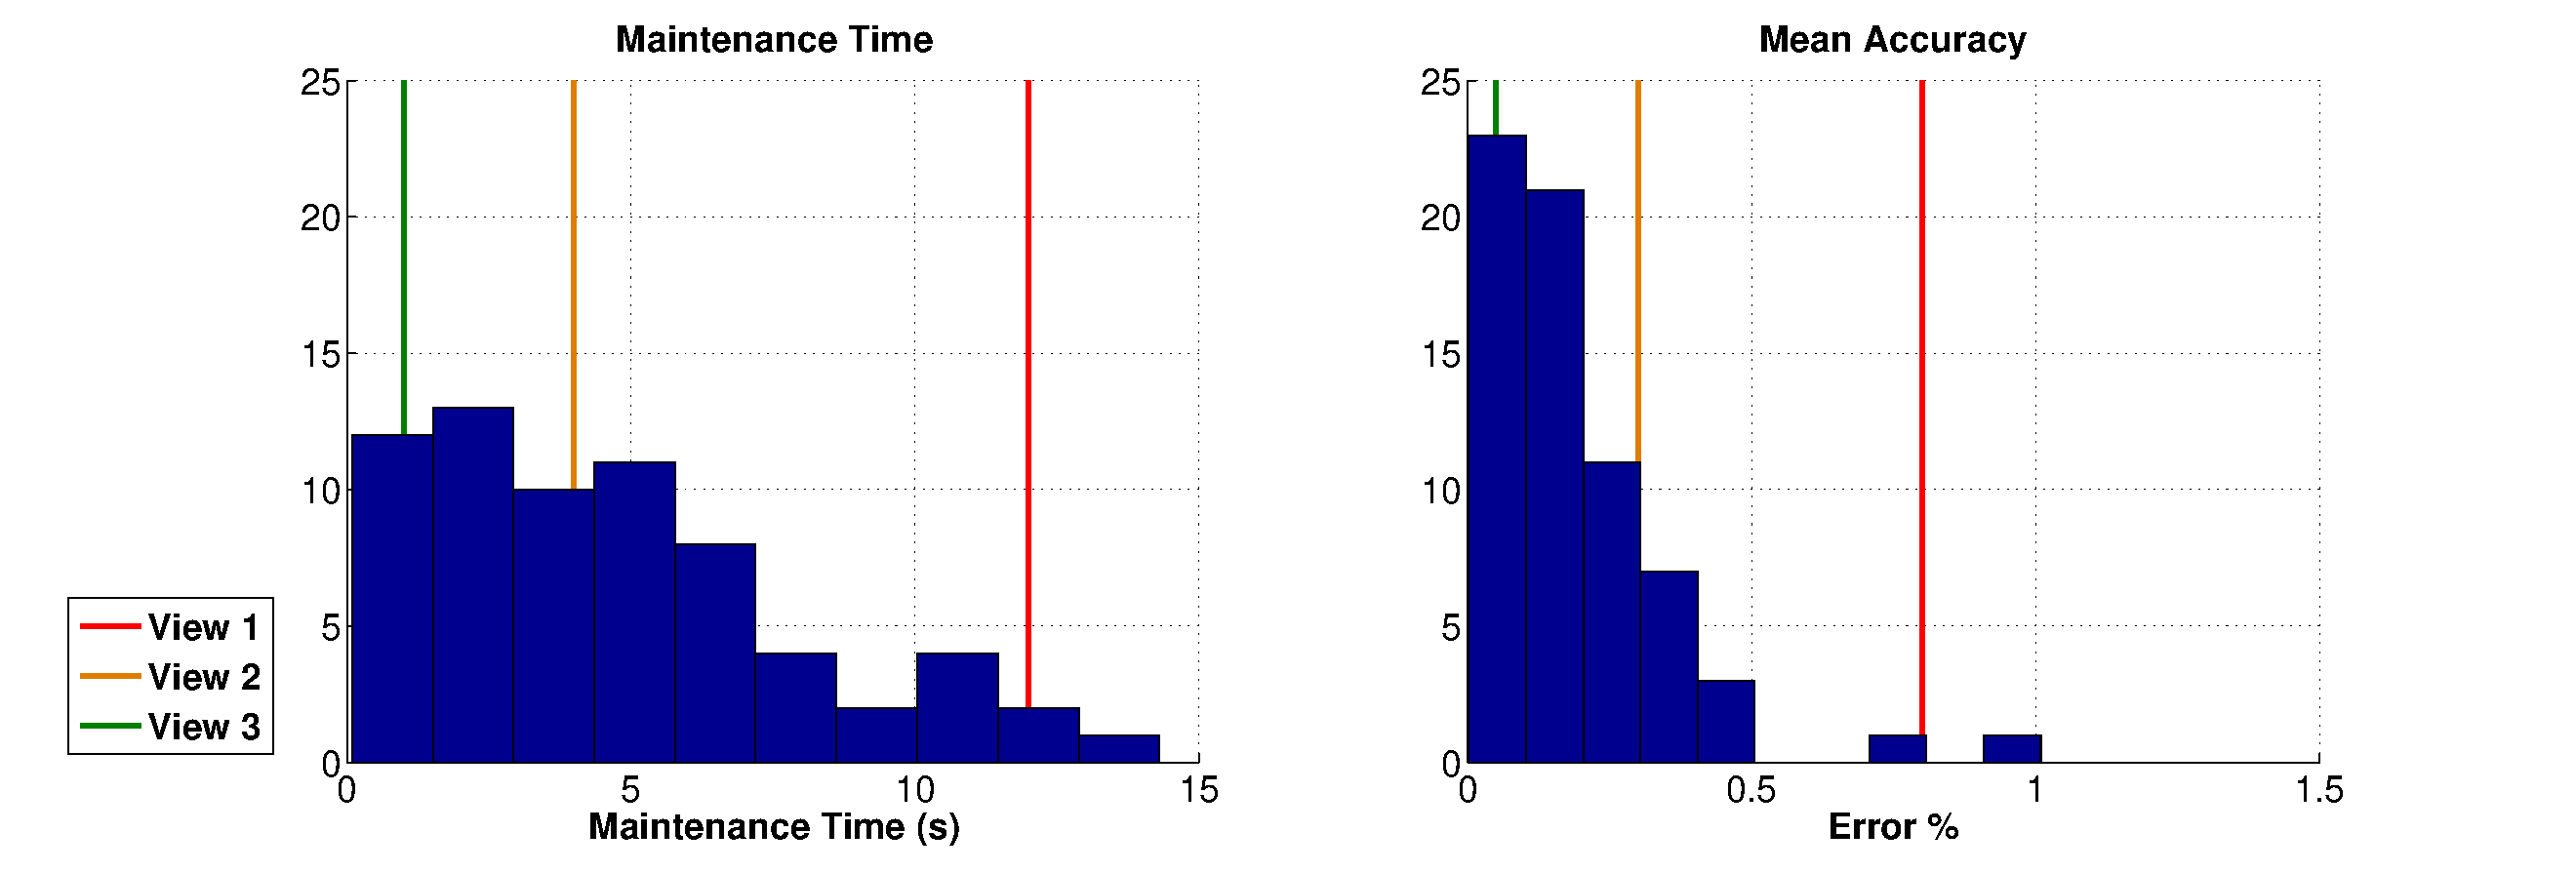
\includegraphics[scale=0.25]{exp/conviva_efficiency_accuracy.eps}
 \caption{We chose three views that represented the distribution of all views well in terms of both accuracy. We plot the staleness of each of the 67 views and mark the three views in our experiment.\label{exp12conviva}}
\end{figure}
For the rest of our experiments, we use SmallView as the counter-example since the results are not affected much by the updates.
Even so, we still show in subsequent experiments that we can acheive more accurate query results and save on maintenance time.

\subsubsection{Accuracy in Conviva}
We evaluated the average query accuracy for different sample sizes and numbers of records inserted.
As before, we derived each view from a 7GB base table and inserted 1.4GB (20\%) of records to the table. 
We built an outlier index on all of the attributes that represent time intervals or rates.
Figure \ref{exp5conviva}, compares the accuracy to the staleness of the query.
We find that even a $0.1\%$ sample gives significantly more accurate results for LargeView and MediumView.
Even in the situation where the view is small, sampling can still have benefits as seen in SmallView.

\begin{figure}[ht!]
\hspace{-3.5em}
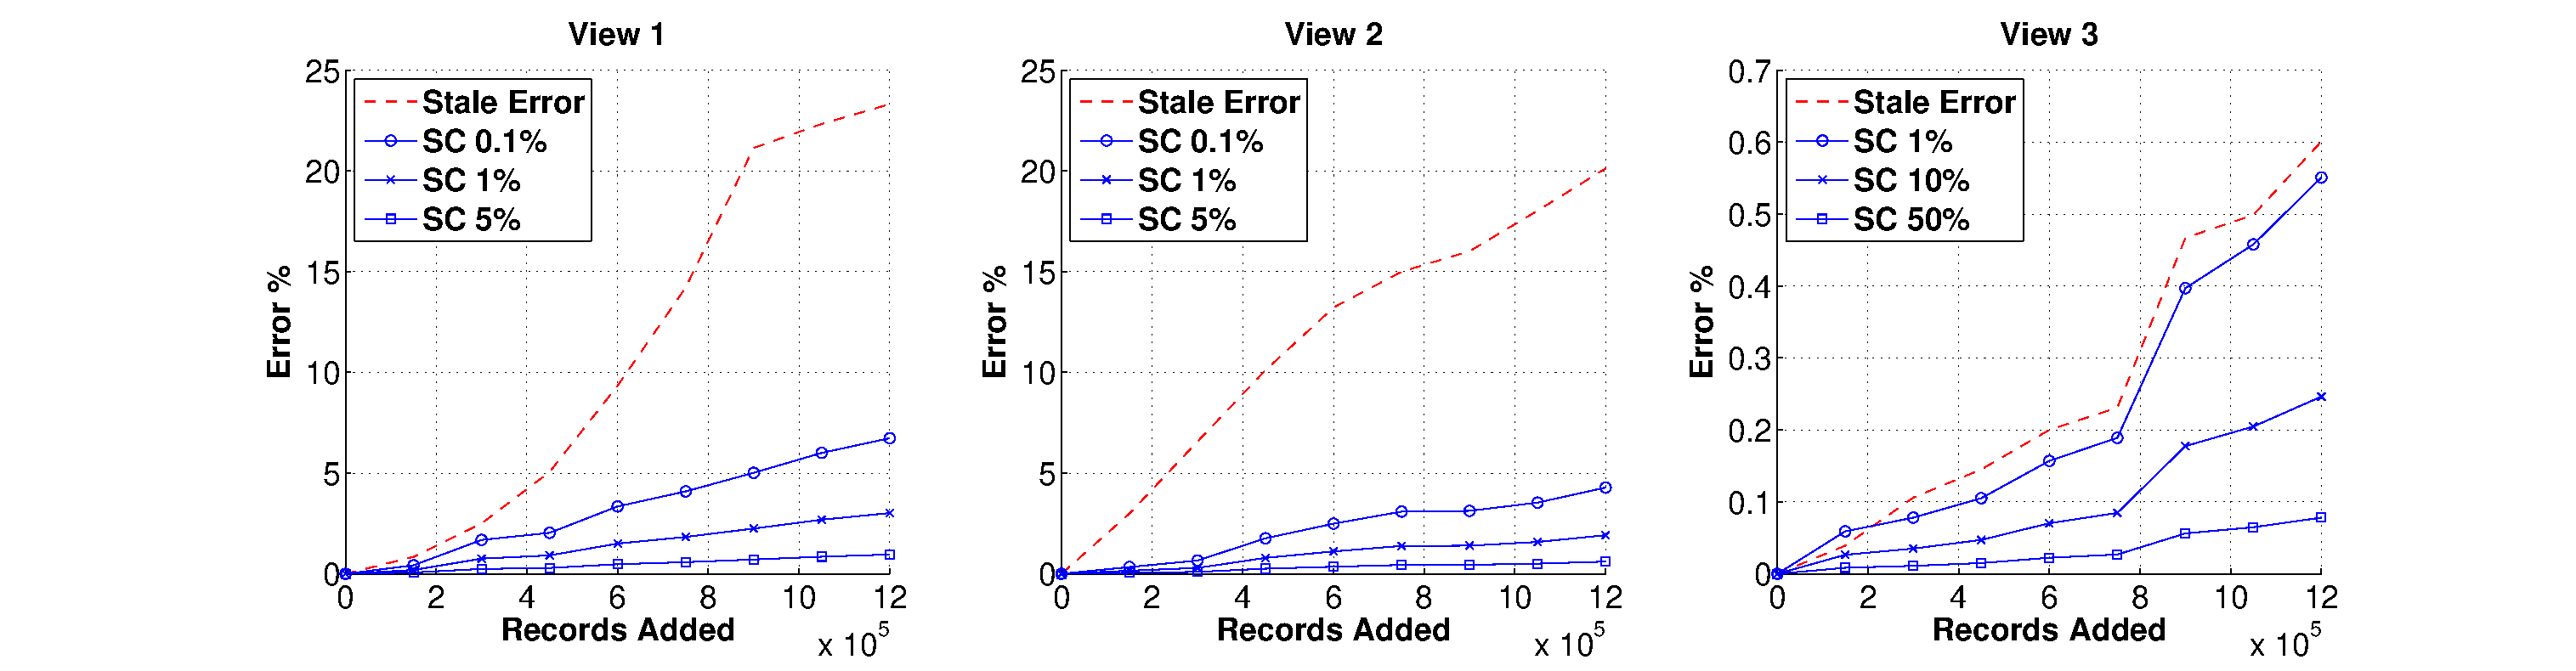
\includegraphics[scale=0.22]{exp/exp5-coniva-accuracy.eps}
 \caption{We compare average query staleness to our approach for a variety of sample sizes. For the larger views, we find that small sample sizes can give accurate results. Larger sample sizes are needed for accurate estimates in SmallView. \label{exp5conviva}}
\end{figure}

\subsubsection{Performance in Conviva}
We scaled these experiments up significantly from the accuracy experiments to illustrate the performance benefits of sampling at a large scale, however, as insertions as a percentage of the base data are the same.
We derived the views from a 700GB base table and inserted records in approximately 14GB increments. 

\begin{figure*}[ht!]

\hspace{-1em}
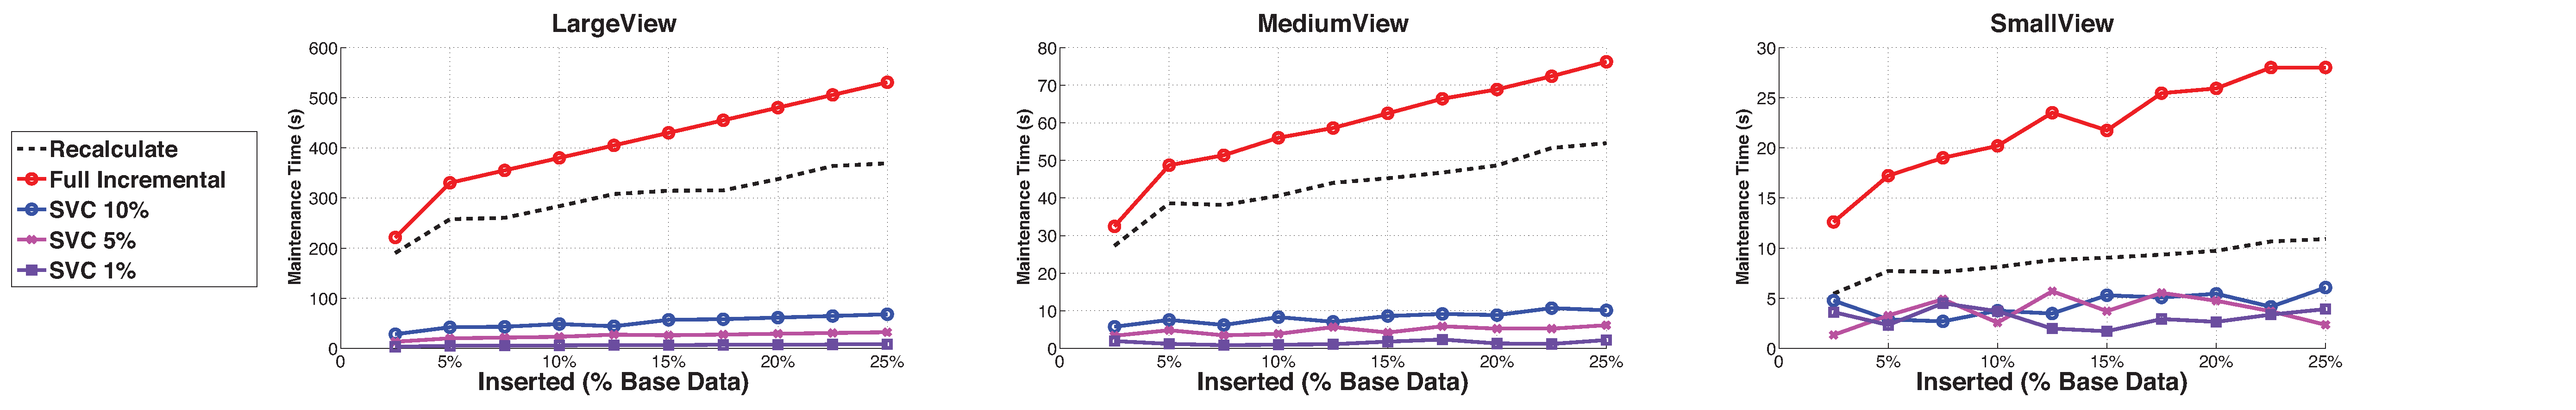
\includegraphics[scale=0.20]{exp/exp5-efficiency-conviva.eps}
 \caption{As before, we compare maintenance times for a variety of sample sizes and full incremental maintenance. We further include a comparision with view recalculation as our experimental platform, Spark, does not support indices or selective writes.\label{exp6conviva}}
\end{figure*}

In Figure \ref{exp6conviva}, we illustrate the maintenance time as a function of the number of inserted records.
As Spark does not support selective writes, we include view recalculation as a baseline for comparision.
In many Spark applications, recalculation is often faster than incremental maintenance.
For LargeView a 10\% sample with 105GB of inserted records (15\%) acheives a  7.5x speedup over full incremental maintenance and a 5.6x speedup over recalculation.
On the other hand, for SmallView, there is a 5.1x speedup over full incremental maintenance and a 1.7x improvement over recalcuation.
Aggregation views with a larger cardinality create larger delta views.
These delta views necessitate a shuffle operation that communications them during the refresh step.
As SmallView is smaller, the communication gains are less and the only savings are in computation.



